In the following section, we will develop the theory behind the Linear-Quadratic Regulator (LQR) based on the theory of \textit{calculus of variations}. We follow the presentation given in \cite{Liberzon2012} by Liberzon closely, but take the basic results relating to Pontryagin's Minimum Principle and the solution to the Algebraic Riccati Equation for granted.

\subsection{Basic Structure of an Optimal Control Problem}\label{subsec:BasicOptimalControl}

We start by sketching the basic structure of an optimal control problem in the language of calculus of variations. Let:

\begin{align}
\dot{x} = &f(x,u,t) \label{eq:BasicOptimalFunction} \\ 
x(t_0) = x_0, \ &x \in \mathbb{R}^n, \ u \in U \in \mathbb{R}^m \label{eq:BasicOptimalDefinitions}
\end{align}

where $t \in \mathbb{R}$ is the time and $x,u$ are functions of $t$, with $U$ the set of admissible controls. We now seek to minimize a cost functional of the type:

\begin{equation}\label{eq:BolzaProblem}
	J = \mathcal{M}(x(T)) + \int_{0}^{T} \mathcal{L}(x(t),u(t)) dt
\end{equation} 

This type of minimization problem is known as a \textit{Bolza problem} and $\mathcal{L}$ is called the \textit{Lagrangian}. To minimize this functional under the constraint of the dynamics in \cref{eq:BasicOptimalDefinitions}, we can formulate a function known as the \textit{Hamiltonian}:

\begin{equation}\label{eq:Hamiltonian}
\mathcal{H}(x(t),u(t),\lambda(t),t) = \lambda^T(t) f(x(t),u(t)) + \lambda_0\mathcal{L}(x(t),u(t))
\end{equation}

where $\lambda^T$ are \textit{Lagrange multipliers} that are commonly referred to as the \textit{costates} of \cref{eq:BasicOptimalFunction} in the context of control. The optimal state, control, and Lagrange multiplier sequences $x^*$, $u^*$, and $\lambda^*$ are then given by Pontryagin's Minimum Principle, which states that the optimal sequences must minimize the Hamiltonian such that:

\begin{equation}\label{eq:MinimizeHamiltonian}
\forall t \in [0,T] \wedge \forall u \in U: \ \mathcal{H}(x^*(t),u^*(t),\lambda^*(t),t) \leq \mathcal{H}(x^*(t),u(t),\lambda^*(t),t)
\end{equation}

while the costates and states must evolve according to each other's respective Hamiltonian gradients:

\begin{align}
	-\dot{\lambda}^T(t) &= \frac{\partial}{\partial x}\mathcal{H}(x^*(t),u^*(t),\lambda(t),t) = \frac{\partial}{\partial x} \Big( \lambda^T f(x^*(t),u^*(t)) + \lambda_0\mathcal{L}(x^*(t),u^*(t)) \Big) \label{eq:LagrangeVariationCondition} \\
	\dot{x} &= \frac{\partial}{\partial \lambda} \mathcal{H}(x^*(t),u^*(t),\lambda(t),t) = \frac{\partial}{\partial \lambda} \Big( \lambda^T f(x^*(t),u^*(t)) + \lambda_0\mathcal{L}(x^*(t),u^*(t)) \Big) \label{eq:StateVariationCondition}
\end{align}

and the costates must fulfil the terminal condition:

\begin{equation}\label{eq:LagrangeTerminalCondition}
 \lambda^T(T) = \mathcal{M}_x(x(T))
\end{equation}

\clearpage

\subsection{The Linear-Quadratic Control Problem}\label{subsec:LQR}

We will now address the well-known LQR problem as a special case of an optimal control problem. Following the same basic problem structure as in \cref{subsec:BasicOptimalControl}, let the dynamics of the system be given by:

\begin{align}
	&\dot{x}(t) = A(t)x(t) + B(t)u(t) \label{eq:TimeVaryingLinearSystem} \\
	&x(t_0) = x_0
\end{align}

and let a cost functional be given by:

\begin{equation}
 J = \int_{t_0}^{t_1} \big(x^T(t)Q(t)x(t) + u^T(t)R(t)u(t)\big)dt + x^T(t_1)\mathcal{M}x(t_1)
\end{equation}

with $Q(t) \wedge \mathcal{M}$ symmetric and positive semidefinite, and $R(t)$ symmetric positive definite. Clearly, this is a Bolza problem with the Lagrangian:

\begin{equation}\label{eq:LQRLagrangian}
\mathcal{L}(x(t),u(t)) = x^T(t)Q(t)x(t) + u^T(t)R(t)u(t)
\end{equation}

and per \cite{Liberzon2012} we may freely choose $\lambda_0 = -1$\footnote{Letting $\lambda_0 = 1$ will simply result in an inverted sign of the optimal gain, and an optimal feedback law of the type $-Kx$ instead of $Kx$.} such that the Hamiltonian becomes:

\begin{equation}\label{eq:LQRHamiltonian}
	\mathcal{H}(x(t),u(t),\lambda(t),t)) = \lambda^T(t)\big(A(t)x(t) + B(t)u(t)\big) - x^T(t)Q(t)x(t) - u^T(t)R(t)u(t)
\end{equation}

Intuitively, the control gradient $\frac{\partial \mathcal{H}}{\partial u}$ of \cref{eq:LQRHamiltonian} must vanish along the optimal control trajectory $u^*(t)$ if we are to satisfy the first condition of Pontryagin's Minimum Principle in \cref{eq:MinimizeHamiltonian}. Taking the partial differential, we obtain:

\begin{equation}\label{eq:HamiltonianUGradient}
 \frac{\partial \mathcal{H}}{\partial u} = B^T(t)\lambda^*(t) - 2R(t)u^*(t)
\end{equation}

and thus it seems clear that $u^*(t)$ must satisfy:

\begin{equation}\label{eq:OptimalControlSequence}
	u^*(t) = \frac{1}{2} R^{-1}(t)B^T(t)\lambda^*(t)
\end{equation}

It can then be shown - doing so is expressly outside the scope of this report, but relies on the remaining conditions \cref{eq:LagrangeVariationCondition,eq:StateVariationCondition,eq:LagrangeTerminalCondition} - that $\lambda^*(t)$ must satisfy a relation of the form:

\begin{equation}\label{eq:OptimalCostateSequence}
	\lambda^*(t) = -2P(t)x^*(t)
\end{equation}

We see that this is quite clearly true at the boundary $t = T$, where per \cref{eq:LagrangeTerminalCondition} we must satisfy that:

\begin{equation}\label{eq:PontryaginBoundaryCondition}
	\lambda^T(T) = \mathcal{M}_x(x(T)) = -2\mathcal{M}x^*(T)
\end{equation}

The relation in \cref{eq:OptimalCostateSequence} then gives a state feedback control law in the form of:

\begin{equation}\label{eq:LQRFeedbackLaw}
	u^*(t) = -R^{-1}(t)B^T(t)P(t)x^*(t)
\end{equation}

and furthermore it can be shown that $P(t)$ evolves according to dynamics known as the \textit{Riccati differential equation}, which are given by:

\begin{equation}\label{eq:RDE}
	\dot{P}(t) = -P(t)A(t) - A^T(t)P(t) - Q(t) + P(t)B(t)R^{-1}(t)B^T(t)P(t)
\end{equation}

\subsection{The Infinite-Horizon Linear-Quadratic Control Problem}\label{subsec:InfiniteHorizonLQR}

We will now narrow down the contents of \cref{subsec:LQR} even further to consider a particularly - and in terms of its solution, rather uniquely beautiful - special case of the LQR problem. Specifically, we will consider the infinite-horizon, time-invariant case with no terminal cost. Thus, let the dynamics be given by:

\begin{align}
	&\dot{x}(t) = Ax(t) + Bu(t) \label{eq:InvariantLinearSystem} \\
	&x(t_0) = x_0
\end{align}

and let the cost functional be:

\begin{equation}\label{eq:LagrangeProblem}
 J = \int_{t_0}^{\infty} \big(x^T(t)Qx(t) + u^T(t)Ru(t)\big)dt
\end{equation} 

In the absence of a terminal cost, this is now known as a \textit{Lagrange problem}. Constructing the Hamiltonian as before, we have:

\begin{equation}\label{eq:InfLQRHamiltonian}
	\mathcal{H}(x(t),u(t),\lambda(t),t)) = \lambda^T(t)\big(Ax(t) + Bu(t)\big) - x^T(t)Qx(t) - u^T(t)Ru(t)
\end{equation}

As before, the control gradient:

\begin{equation}\label{eq:HamiltonianUGradientInfLQR}
	\frac{\partial \mathcal{H}}{\partial u} = B^T\lambda^*(t) - 2Ru^*(t)
\end{equation}

must vanish along the optimal trajectory, necessitating that:

\begin{equation}\label{eq:OptimalControlSequence}
	u^*(t) = \frac{1}{2} R^{-1}B^T\lambda^*(t)
\end{equation}

and it can analogously to \cref{subsec:LQR} be shown that:

\begin{equation}\label{eq:OptimalCostateSequenceInfLQR}
	\lambda^*(t) = -2Px^*(t)
\end{equation}

such that:

\begin{equation}\label{eq:InfLQRFeedbackLaw}
	u^*(t) = -R^{-1}B^TPx^*(t)
\end{equation}

with $P$ now time-invariant and fulfilling the \textit{algebraic Riccati equation}:

\begin{equation}\label{eq:ARE}
	 PA + A^TP + Q - PBR^{-1}B^TP = 0
\end{equation}

This motivates the - frankly somewhat stunning - conclusion that for the infinite-horizon, time-invariant LQR problem, the optimal state feedback law may be calculated \textit{entirely} offline.

A final important result concerns the global stability of this feedback law. Let an auxiliary equation to \cref{eq:InvariantLinearSystem} be given by:

\begin{equation}\label{eq:OutputEquation}
	y = Cx
\end{equation}

then choosing $Q = C^TC$ such that the cost functional becomes:

\begin{equation}\label{eq:ExpoStableLagrangeProblem}
	J(u) = \int_{t_0}^{\infty} \big(x^T(t)C^TCx(t) + u^T(t)R(t)u(t)\big)dt
\end{equation} 

\textit{guarantees} exponential stability of the closed-loop system $\dot{x}^* = (A-BR^{-1}B^TP)x^*$ so long as $(A,C)$ are an observable pair \cite{Liberzon2012}.

\subsection{Tracking LQR and Integral Action}\label{subsec:TrackingAndIntegralAction}

The aware reader will have noted that the preceding sections in \cref{sec:LQR} strictly address \textit{regulator} problems - i.e., the regulation of a system to the origin. In practice, this is rarely a sufficient problem definition for practical purposes, as most systems have some setpoint or other. 

Fortunately, casting the Lagrange problem in \cref{eq:LagrangeProblem} as a tracking problem is largely trivial, as we may simply choose a new coordinate system with the target as the origin. We may perform a similar coordinate shift on the control to specify a desired operating point. For convenience of notation, we let $\hat{x} = x-x_r$ and $\hat{u} = u-u_r$ and take the time index $t$ to be implicit. Then we can represent the Lagrange problem in the shifted coordinate system as:

\begin{equation}\label{eq:LagrangeProblemSetpoint}
	J = \int_{t_0}^{\infty} \big(\hat{x}^TQ\hat{x} + \hat{u}^TR\hat{u}\big)dt
\end{equation} 

We can by a similar ploy convert \cref{eq:LagrangeProblemSetpoint} into an \textit{output} tracking problem, which is perhaps the most common practical control problem, as $C$ is simply a linear transformation on the states:

\begin{equation}\label{eq:LagrangeProblemOutput}
	J = \int_{t_0}^{\infty} \big((C\hat{x})^TQ_y(C\hat{x}) + \hat{u}^TR\hat{u}\big)dt = \int_{t_0}^{\infty} \big(\hat{y}^TQ_y\hat{y} + \hat{u}^TR\hat{u}\big)dt
\end{equation} 

We now note that as with many other state-space control algorithms, an LQR controller does not inherently have integral action. There are multiple ways of adding this to LQR, such as the classical integrator state approach \cite{Skogestad2005}. Here the extended state $\bar{x} = [x \ x_i]^T$ is defined, and the system evolves according to the dynamics:

\begin{align}\label{eq:ClassicalIntegralAction}
&u = -\bar{K}\bar{x} \\
&\dot{\bar{x}} = \bar{A}\bar{x} + \bar{B}u + B_r r \\ 
&y = \bar{C}\bar{x} \\
&\bar{A} = \begin{bmatrix}A & 0 \\ -C & 0 \end{bmatrix}, \ \bar{B} = \begin{bmatrix} B \\ 0 \end{bmatrix}, \ B_r = \begin{bmatrix} 0 \\ 1 \end{bmatrix}, \ \bar{C} = \begin{bmatrix} C & 0 \end{bmatrix},
\ \bar{K} = -\begin{bmatrix} K & -K_i \end{bmatrix},
\end{align}

This approach, however, introduces the issue of weighting $x_i$ appropriately. This can be an awkward weight to choose, as the state represents the time integral of the tracking error, rather than the tracking error directly. We therefore prefer an alternative integral action design, which we describe in \cref{subsec:VelocityFormLQR}.

\subsection{The Velocity-Form LQR Algorithm}\label{subsec:VelocityFormLQR}

We will now present the velocity-form LQR algorithm, as detailed in \cite{Pannocchia2001,Ruscio2012}. We will make the initial assumption that the system dynamics have been discretised by some appropriate method, and we then define the deviation variables:

\begin{equation}\label{eq:VelocityVariables}
	\Delta x_k = x_k - x_{k-1}, \ \Delta y_k = y_k - r_k, \ \Delta u_k = u_k-u_{k-1}
\end{equation}

where $k$ is the sample index. We then define the extended vectors and matrices:

\begin{equation}\label{eq:VelocityMatrices}
	\tilde{x}_k = \begin{bmatrix} \Delta x_k \\ \Delta y_k	\end{bmatrix}, \ \tilde{u}_k = \Delta u_k, \
	\tilde{A} = \begin{bmatrix} A & 0 \\ CA & I	\end{bmatrix}, \ 
	\tilde{B} = \begin{bmatrix} B \\ CB	\end{bmatrix}, \ \tilde{C} = \begin{bmatrix} 0 & I	\end{bmatrix}
\end{equation}

and the velocity-form dynamics:

\begin{align}\label{eq:VelocityDynamics}
	&\tilde{x}_{k+1} = \tilde{A}\tilde{x}_k + \tilde{B}\tilde{u}_k \\
	&\Delta y_k = \tilde{C}\tilde{x}_k \\
\end{align}

We now note a number of interesting properties about this velocity-form algorithm. Consider first the origin regulation problem, i.e. $\tilde{x} \rightarrow 0$. Clearly, driving $\tilde{x}$ to $0$ must drive the system to settle at exactly $r$, per the definitions in \cref{eq:VelocityVariables}, as:

\begin{equation}\label{eq:VelocityDriveToOrigin}
	\begin{split}
		&\tilde{x} = 0 \Rightarrow \Delta x = 0 \\ 
		&\tilde{x} = 0 \Rightarrow \Delta y = 0 \Rightarrow y = r
	\end{split}
\end{equation}

Consider now the discretized Lagrange problem phrased in terms of these deviation variables:

\begin{equation}\label{eq:LagrangeProblemDeviation}
	J = \sum_{k_0}^{\infty} \big(\tilde{x}^TQ\tilde{x} + \tilde{u}^TR\tilde{u}\big) = \sum_{k_0}^{\infty}\left( \begin{bmatrix} \Delta x_k \\ \Delta y_k\end{bmatrix}^T Q
	\begin{bmatrix} \Delta x_k \\ \Delta y_k\end{bmatrix} + 
	\Delta u_k^TR\Delta u_k \right)
\end{equation} 

Clearly, this functional penalizes deviations from the origin of the state space, which is located exactly at $\{0,0,r\}$, while penalizing deviations from the default control input of $0$. Consider now the case of an arbitrary linearisation around some equilibrium point $x_{e}$ and corresponding operating point $u_{op}$. A linearization of this type will take the form:

\begin{equation}\label{eq:LinearizationAroundOP}
	\begin{split}
	&f(x,u) \approx \frac{\partial f}{\partial x} \tilde{x} + \frac{\partial f}{\partial u} \tilde{u}, \\ 
	&\tilde{x} = x-x_e, \ \tilde{u} = u - u_{op}
	\end{split}
\end{equation}

which lends itself to the interpretation that:

\begin{equation}\label{eq:DeltaInterpretation}
	\Delta \tilde{x} = x-x_e, \ \Delta \tilde{u} = u-u_{op}
\end{equation}

\clearpage

This is a quite attractive quality when contextualised by the Hartman-Grobman theorem, as we expect linearised model dynamics to closely\footnote{Exactly, in fact, in some indeterminately sized region} approximate the real system dynamics in some region around the equilibrium point $\{x_e,u_{op}\}$, and the velocity LQR algorithm will penalize deviations from the point $\{x_e,u_{op},r\}$, thus regulating the system to $r$ while deviating minimally from the vicinity of the equilibrium $\{x_e,u_{op}\}$.

We note additionally - and importantly - that the control law resulting from \cref{eq:LagrangeProblemDeviation} is a control \textit{increment} law, i.e. that:

\begin{equation}\label{eq:ControlIncrementLaw}
	\Delta u^*(k) = -\Delta K(k) \Delta x(k) 
\end{equation}

and that the actual control applied to the system at any time $k$ is:

\begin{equation}\label{eq:ActualControlApplied}
	\begin{gathered}
		\Delta u^*(k) = -\Delta K(k)x(k) \\
		u^*(k) = \sum_{i=1}^{k} \Delta u^*(i)
	\end{gathered}
\end{equation}

\subsection{Disturbance-Accommodating Linear Quadratic Regulator for Exogenous Inputs}\label{subsec:DALQR}

We now address a final LQR-related wrinkle. As shown in \cref{eq:TankPressureStateSpace}, the consumer demand flows are modelled as exogenous, uncontrolled inputs. Standard LQR does not accommodate this construction, but may be modified to accommodate exogenous inputs by adding an additional term to the optimal control law \cite{Singh2017} such that:


\begin{equation}\label{eq:ELQRControlLaw}
	u(k) = u^*(k) - B^\dagger B \delta(k)
\end{equation}

where $B^\dagger$ is the Moore-Penrose pseudoinverse of $B$ and $\delta(k)$ is the exogenous input at time $k$.

\subsection{Implementation and Simulation Study}\label{subsec:LQRSimulationStudy}

In this section, we detail the implementation and simulation study of a velocity-form LQR controller for the tank pressure dynamics described by \cref{eq:TankPressureStateSpace}. We choose a discretisation time $t_s = 100 \si{s}$, and the tank constant is $\tau = -0.000096 \frac{\si{bar}}{\si{m^3}}$, such that $T = 0.0096$. This results in the system:

\begin{equation}\label{eq:TankPressureMatrices}
	\begin{gathered}
		p_\tau(k+1) = A p_\tau(k) + B_p d_p(k) + B_c d_c(k)  \\
		A = 1, \ B_p = B_c = [0.0096 \ 0.0096], \ C = 1 ,
	\end{gathered}
\end{equation}

Using the velocity-form transform from \cref{eq:VelocityMatrices}, the system becomes:

\begin{equation}\label{eq:TankPressureVelocityMatrices}
\begin{gathered}
	 \begin{bmatrix}\Delta	p_\tau(k+1) \\\ p_\tau(k+1)-p_{r}
	\end{bmatrix} = \tilde{A} \Delta p_\tau(k) + \tilde{B}_p \Delta d_p(k) + \tilde{B}_c \Delta d_c(k)  \\
	\tilde{A} = \begin{bmatrix} 1 & 0 \\ 1 & 1 \end{bmatrix},
	 \ \tilde{B}_p = \tilde{B}_c = \begin{bmatrix} 0.0096 & 0.0096 & \\ 0.0096 & 0.0096\end{bmatrix}, \ \tilde{C} = [0 \ 1]	
\end{gathered}
\end{equation}

\clearpage

We now simulate the system under a variety of conditions, including significant model error and an output disturbance. In every case, a significant state disturbance is applied to the system.

\begin{figure}[h!]
	\centering
	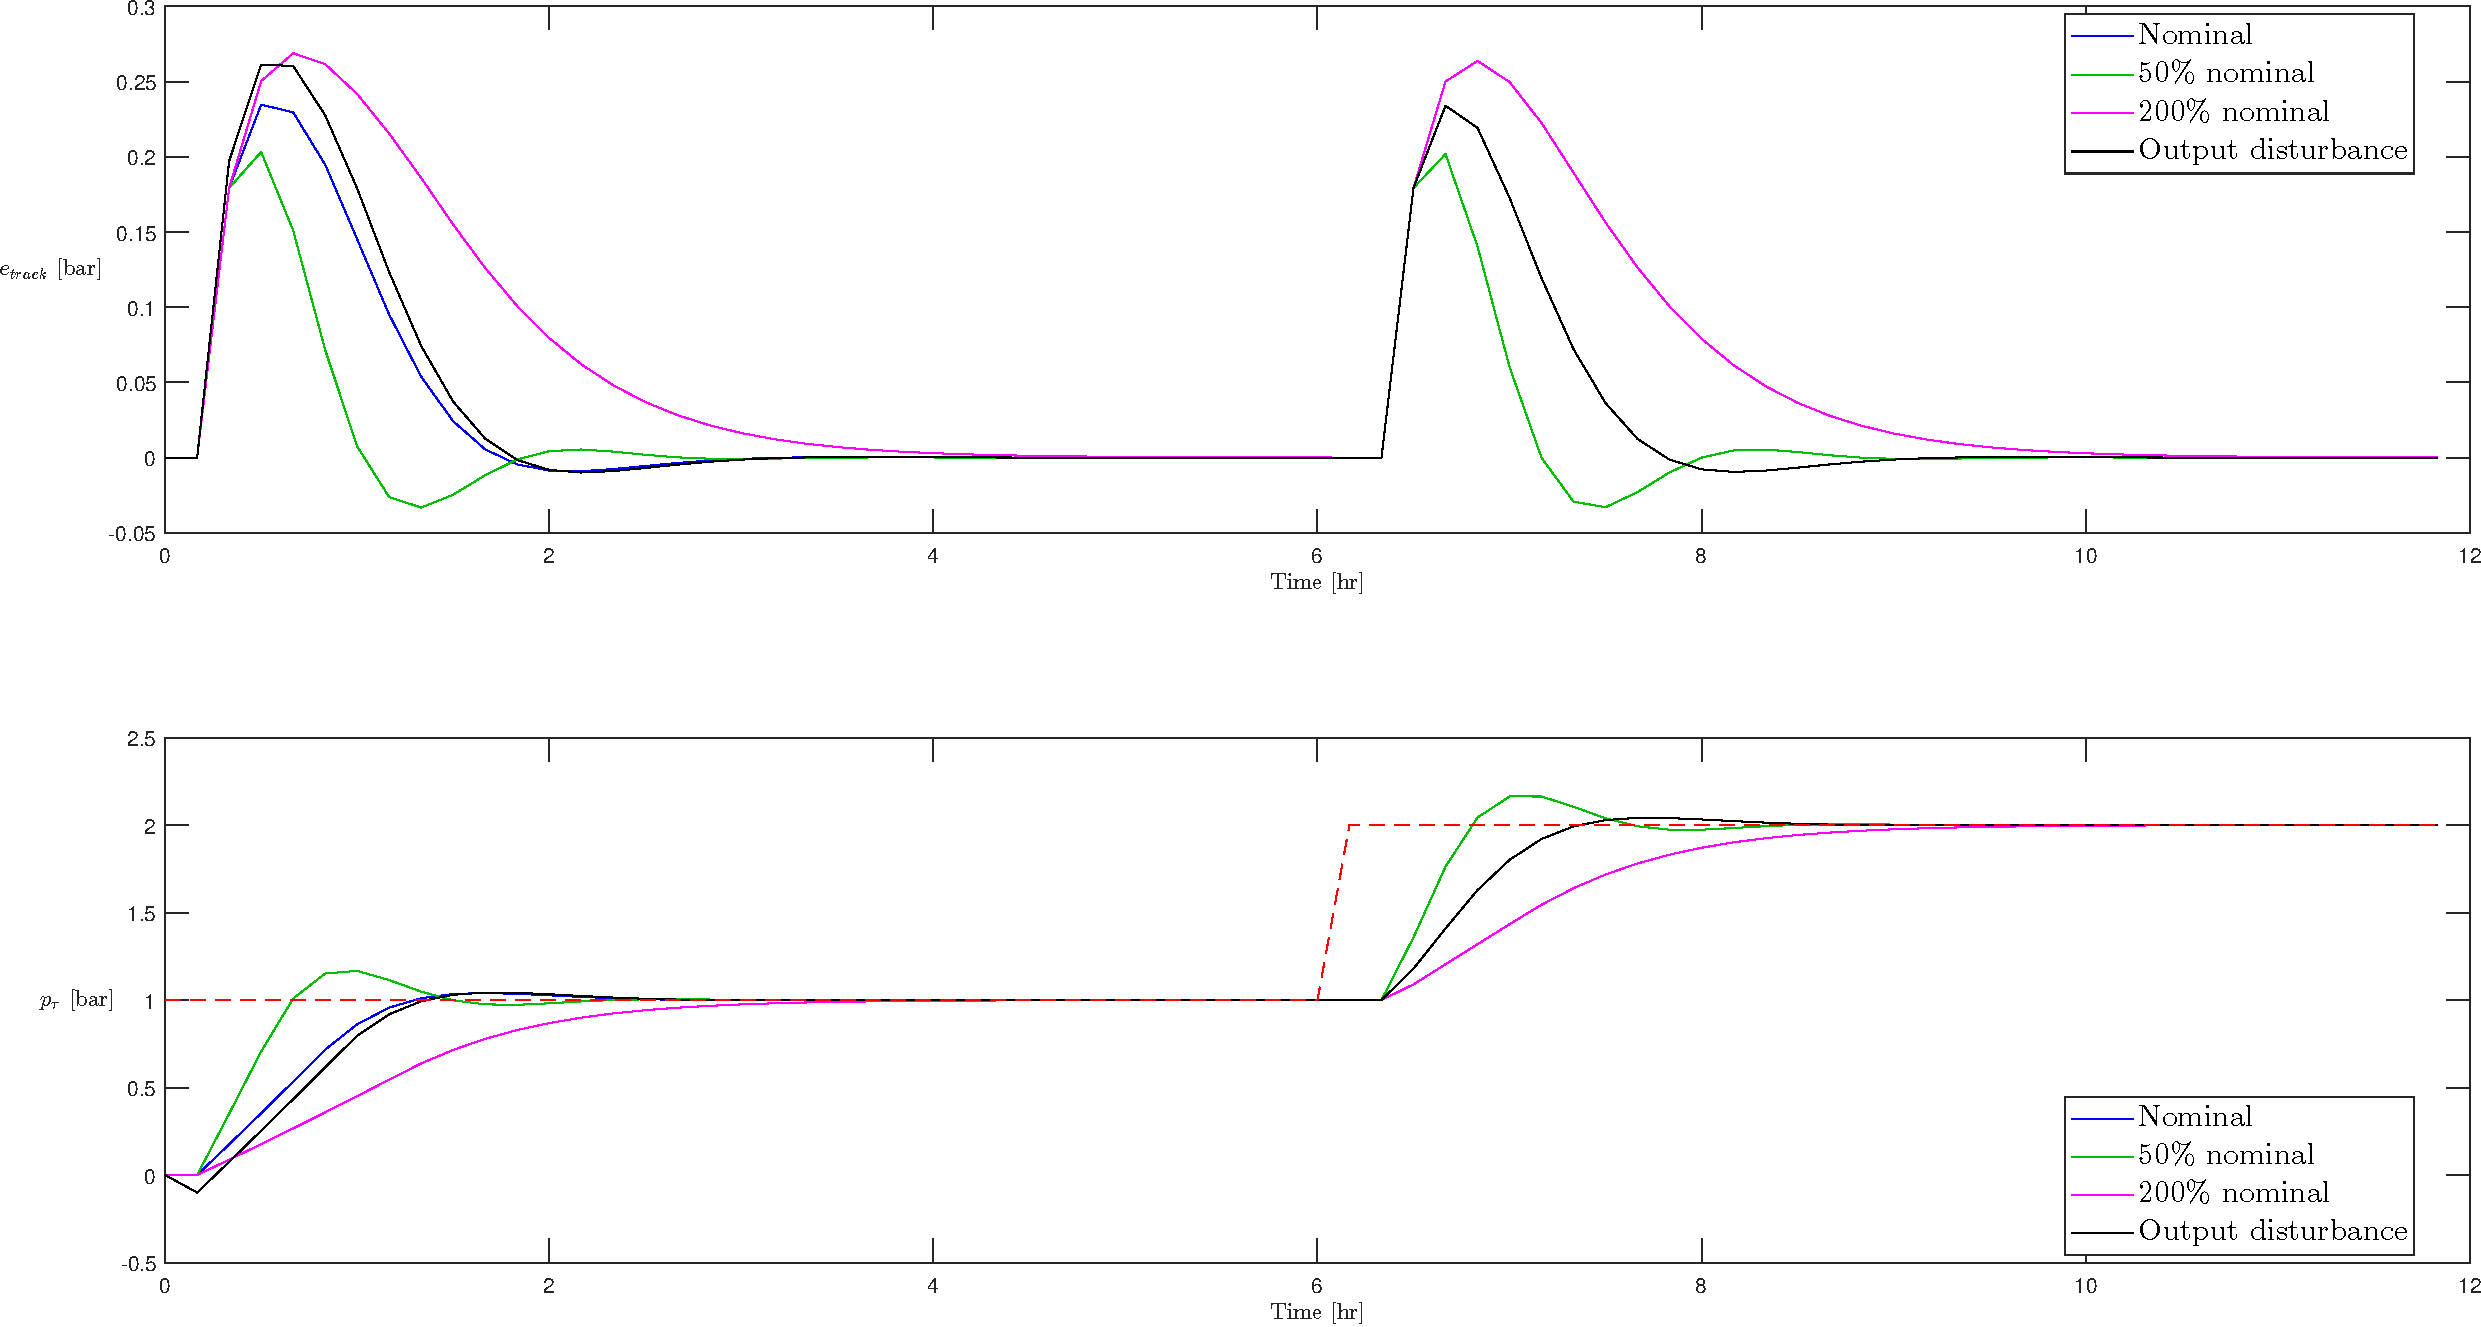
\includegraphics[width=0.8\textwidth]{Pictures/LQRTracking.pdf}
	\caption{Tracking performance of the VF-LQR controller}
	\label{fig:LQRTracking}
\end{figure}

It is clear that the proposed controller is capable of compensating for the disturbance and tracking, even under significant model error or output disturbance.

\begin{figure}[h!]
	\centering
	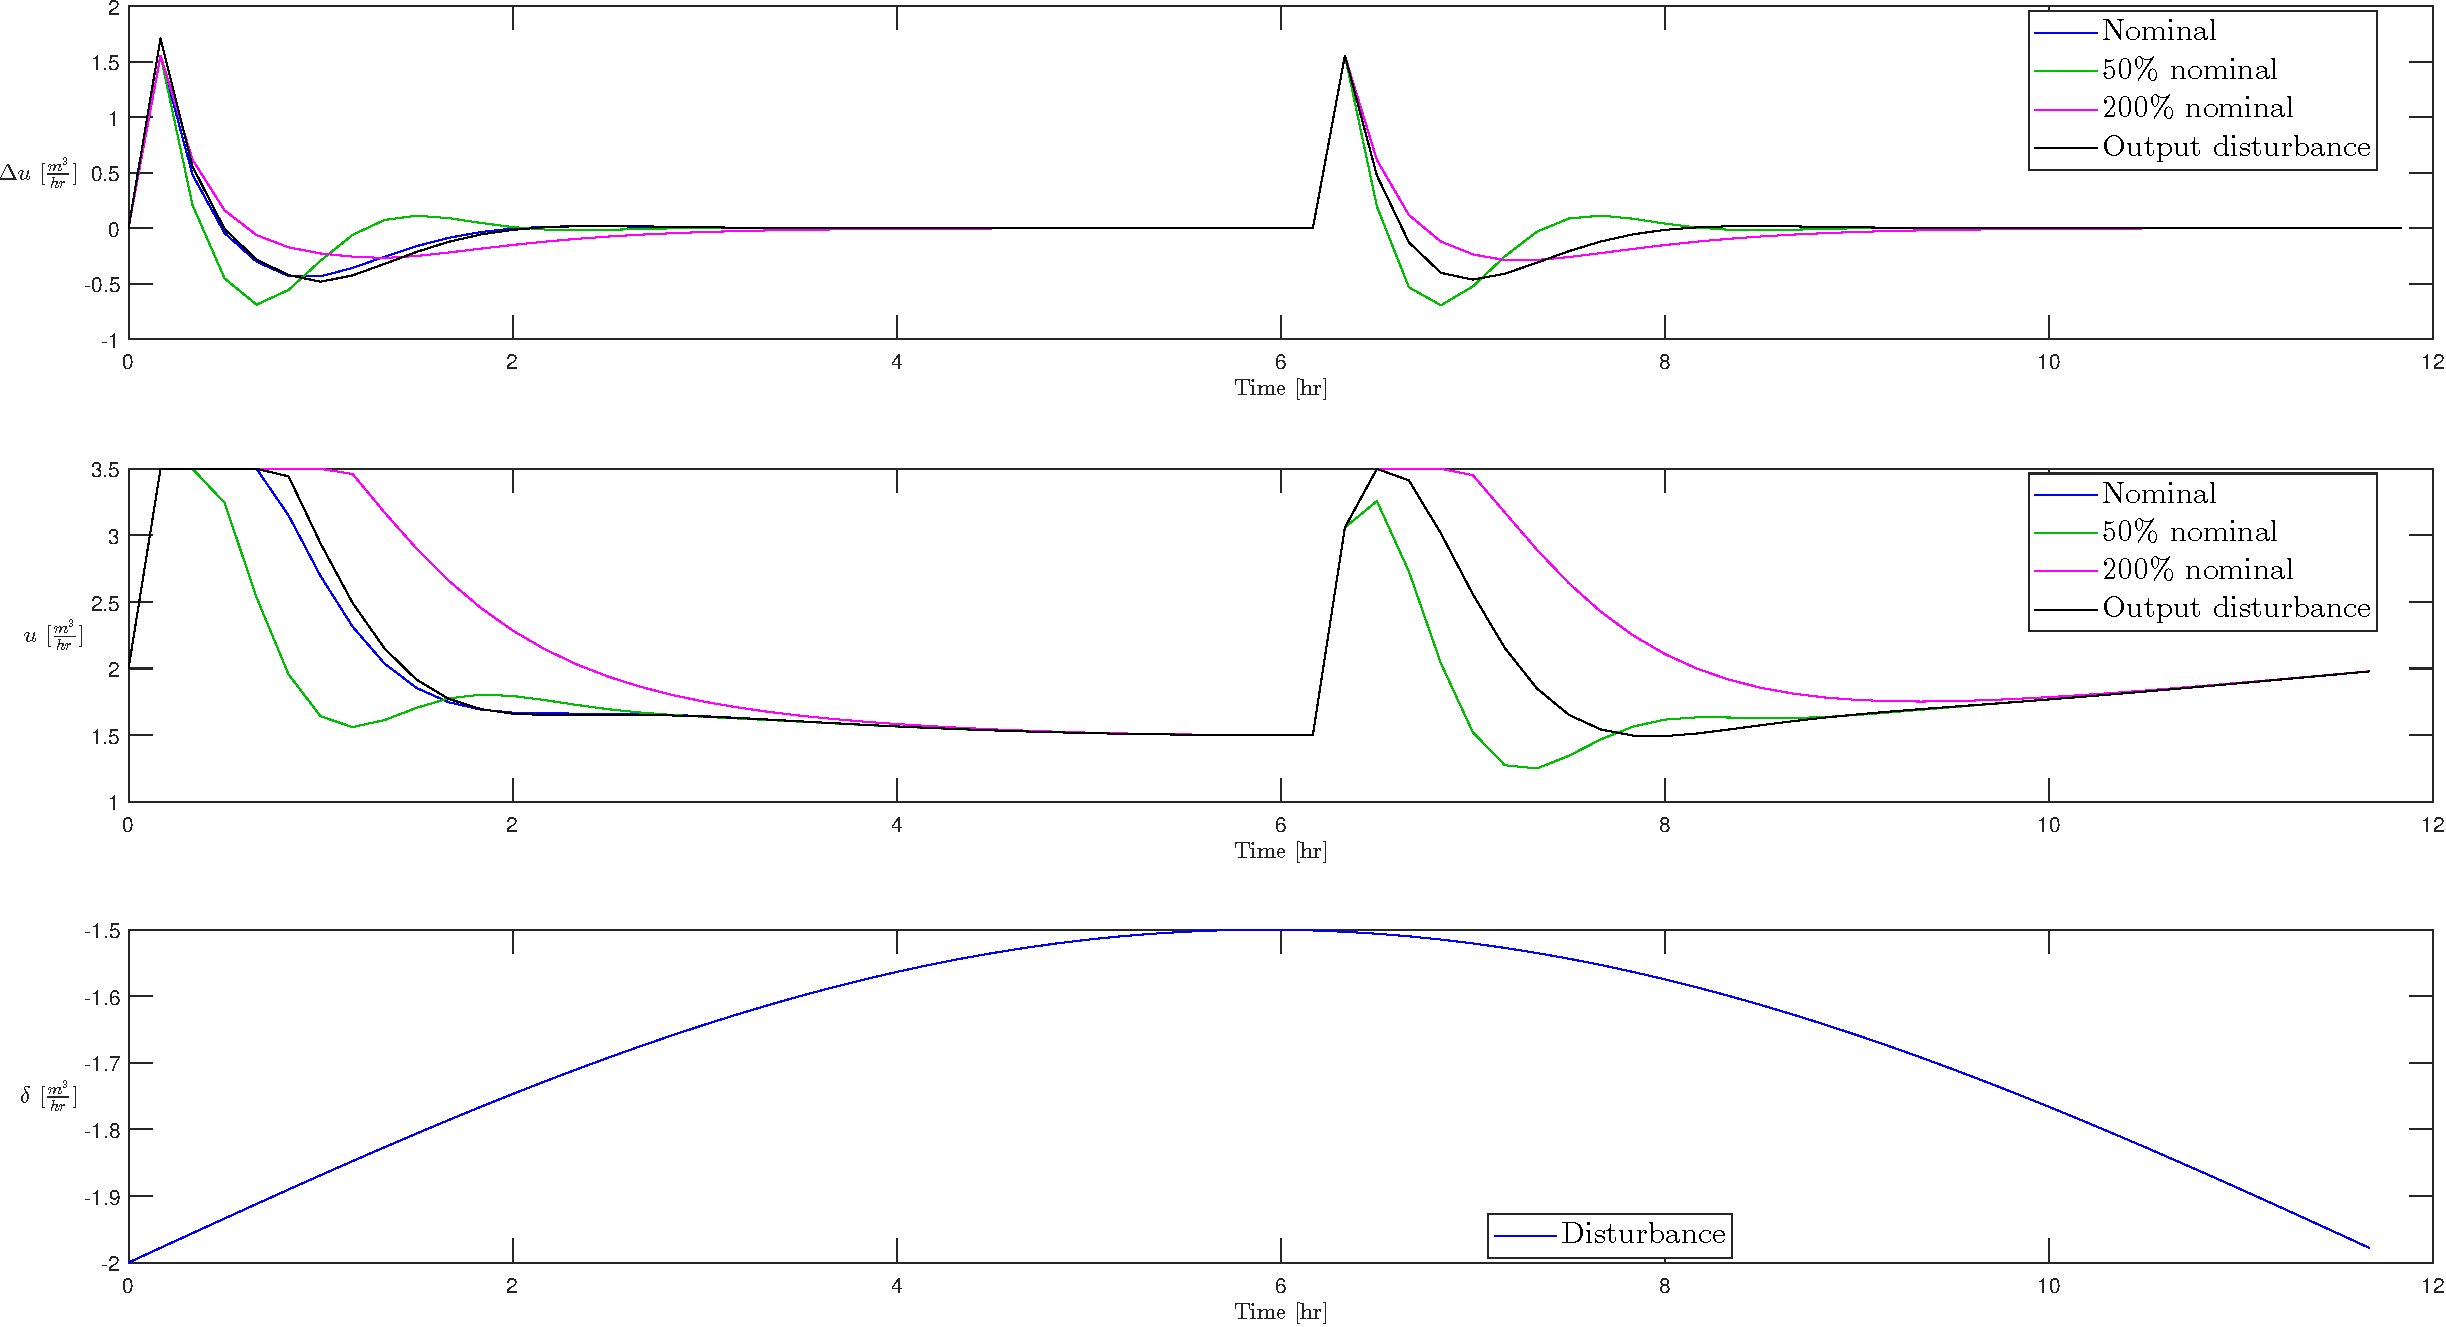
\includegraphics[width=0.8\textwidth]{Pictures/LQRControls.pdf}
	\caption{Control effort of the VF-LQR controller}
	\label{fig:LQRControls}
\end{figure}

We see on \cref{fig:LQRControls} that rejection of the state disturbance is, as expected based on \cref{eq:ELQRControlLaw}, accomplished by reverse-phase injection of the disturbance signal. This also reveals a fundamental limitation of VF-LQR with the proposed disturbance rejection strategy; its tracking ability is asymptotically bounded by the steady-state error in the disturbance estimate.


